
\documentclass[12pt,a4paper]{report}
\usepackage{dissertation}
\usepackage{pgfgantt}
\makeglossaries
\makeindex

\logo{EE}{School of Engineering}{}
\logoB{EE}{School of Engineering}{}

\author{Your Name Here}

\titleA{The Socioeconomic Impact of Duck-Sized}
\titleB{Horses in Urban Environments}


\usepackage[toc,page]{appendix}
\usepackage{pgfplots}
\usepackage{pgf-pie}
\usepackage{algorithm}% http://ctan.org/pkg/algorithms
\usepackage{algpseudocode}% http://ctan.org/pkg/algorithmicx
\usepackage{booktabs}

\usepackage{tikz}
\usetikzlibrary{mindmap,trees}

\renewcommand{\baselinestretch}{1}
\bibliographystyle{plainnat}

\begin{document}
\setlength{\parindent}{0em}

%-- Covers
\begin{titlepage}
\color{PANTONECoolGray7C}
\thelogo
\leading{20.4pt}
{\Large
\theauthor
\\
%
\\
\textbf{\thetitleA}
\\
\textbf{\thetitleB}
\\
\textbf{\thetitleC}
}

\vspace*{\fill}
{\footnotesize \myear}
\end{titlepage}

\null
\thispagestyle{empty}
\pagecolor{PANTONECoolGray7C}
\afterpage{\nopagecolor}
\newpage

\begin{titlepage}
\color{PANTONECoolGray7C}
\thelogoB
\leading{20.4pt}
{\Large
\theauthor
\\
%
\\
\textbf{\thetitleA}
\\
\textbf{\thetitleB}
\\
\textbf{\thetitleC}
}

\vspace{55.2mm}
\leading{16.8pt}
{\large
Masters Dissertation
\\
\themasters
\\
\thearea
Dissertation supervised by
\\
\textbf{\thesupervisor}
\\
\thecosupervisor}

\vspace*{\fill}
{\footnotesize \myear}
\end{titlepage}

%-- Document setup
\newgeometry{right=25mm, left=25mm, top=25mm, bottom=25mm}
\pagenumbering{roman}

\setlength{\parskip}{0pt}
\setlength{\parindent}{1.5em}

%-- Preamble
\chapter*{Copyright and Terms of Use for Third Party Work}
\setlength{\parskip}{1em}
\noindent
This dissertation reports on academic work that can be used by third parties as long as the internationally accepted standards and good practices are respected concerning copyright and related rights.

\noindent
This work can thereafter be used under the terms established in the license below.

\noindent
Readers needing authorization conditions not provided for in the indicated licensing should contact the author through the RepositóriUM of the University of Minho.

\section*{License granted to users of this work:}

% \textit{[Caso o autor pretenda usar uma das licenças Creative Commons, deve escolher e deixar apenas um dos seguintes ícones e respetivo lettering e URL, eliminando o texto em itálico que se lhe segue. Contudo, é possível optar por outro tipo de licença, devendo, nesse caso, ser incluída a informação necessária adaptando devidamente esta minuta]}

% \noindent
% 
\includegraphics[]{images/CCBY.png}
% \\
% \textbf{CC BY}
% \\
% \url{https://creativecommons.org/licenses/by/4.0/}
% \textit{[Esta licença permite que outros distribuam, remixem, adaptem e criem a partir do seu trabalho, mesmo para fins comerciais, desde que lhe atribuam o devido crédito pela criação original. É a licença mais flexível de todas as licenças disponíveis. É recomendada para maximizar a disseminação e uso dos materiais licenciados.]}

% %--

% \noindent
% 
\includegraphics[]{images/CCBYSA.png}
% \\
% \textbf{CC BY-SA}
% \\
% \url{https://creativecommons.org/licenses/by-sa/4.0/}
% \textit{[Esta licença permite que outros remisturem, adaptem e criem a partir do seu trabalho, mesmo para fins comerciais, desde que lhe atribuam o devido crédito e que licenciem as novas criações ao abrigo de termos idênticos. Esta licença costuma ser comparada com as licenças de software livre e de código aberto «copyleft». Todos os trabalhos novos baseados no seu terão a mesma licença, portanto quaisquer trabalhos derivados também permitirão o uso comercial. Esta é a licença usada pela Wikipédia e é recomendada para materiais que seriam beneficiados com a incorporação de conteúdos da Wikipédia e de outros projetos com licenciamento semelhante.]}

%--

% \noindent
% 
\includegraphics[]{images/CCBYND.png}
% \\
% \textbf{CC BY-ND}
% \\
% \url{https://creativecommons.org/licenses/by-nd/4.0/}
% \textit{[Esta licença permite que outras pessoas usem o seu trabalho para qualquer fim, incluindo para fins comerciais. Contudo, o trabalho, na forma adaptada, não poderá ser partilhado com outras pessoas e têm que lhe ser atribuídos os devidos créditos.]}

%--

\noindent

\includegraphics[]{images/CCBYNC.png}
\\
\textbf{CC BY-NC}
\\
\url{https://creativecommons.org/licenses/by-nc/4.0/}
% \textit{[Esta licença permite que outros remisturem, adaptem e criem a partir do seu trabalho para fins não comerciais, e embora os novos trabalhos tenham de lhe atribuir o devido crédito e não possam ser usados para fins comerciais, eles não têm de licenciar esses trabalhos derivados ao abrigo dos mesmos termos.]}

%--

% \noindent
% 
\includegraphics[]{images/CCBYNCSA.png}
% \\
% \textbf{CC BY-NC-SA}
% \\
% \url{https://creativecommons.org/licenses/by-nc-sa/4.0/}
% \textit{[Esta licença permite que outros remisturem, adaptem e criem a partir do seu trabalho para fins não comerciais, desde que lhe atribuam a si o devido crédito e que licenciem as novas criações ao abrigo de termos idênticos.]}

% %--

% \noindent
% 
\includegraphics[]{images/CCBYNCND.png}
% \\
% \textbf{CC BY-NC-ND}
% \\
% \url{https://creativecommons.org/licenses/by-nc-nd/4.0/}
% \textit{[Esta é a mais restritiva das nossas seis licenças principais, só permitindo que outros façam download dos seus trabalhos e os compartilhem desde que lhe sejam atribuídos a si os devidos créditos, mas sem que possam alterá- los de nenhuma forma ou utilizá-los para fins comerciais.]}

\setlength{\parskip}{0em}
\chapter*{Acknowledgements}
\setlength{\parskip}{1em}

Grateful to obsitex for converting the markdown files to LaTeX.

\setlength{\parskip}{0em}
\chapter*{Statement of Integrity}
\setlength{\parskip}{1em}
\noindent
I hereby declare having conducted this academic work with integrity.

\noindent
I confirm that I have not used plagiarism or any form of undue use of information or falsification of results along the process leading to its elaboration.

\noindent
I further declare that I have fully acknowledged the Code of Ethical Conduct of the University of Minho.

\phantom{space}

\noindent
University of Minho, Braga, \myear

\vspace{25mm}
\noindent\theauthor
\setlength{\parskip}{0em}
\chapter*{Abstract}

An abstract that isn't defined in the markdown file, but could be.

\cleardoublepage


\phantomsection
\tableofcontents

\cleardoublepage
\listoffigures

% List of tables
\renewcommand*{\listtablename}{List of Tables}
\listoftables
\clearpage

% Acronyms
\printglossary[type=\acronymtype,nonumberlist, title={Acronyms}]

% Glossary
\printglossary[title={Glossary}, nonumberlist]

\cleardoublepage
\pagenumbering{arabic}

%-- Dissertation 
\part{Introduction and Background}\label{sec:Introduction_and_Background}

\chapter{Introduction}\label{sec:Introduction}

Urban environments are dynamic ecosystems in which the introduction of novel elements can significantly influence social, economic, and infrastructural development. While the presence of large animals in cities has long been regulated, the potential introduction of duck-sized horses presents unique challenges and opportunities. This study investigates how such creatures could shape urban life, exploring issues such as public perception, economic viability, and potential uses.



\begin{figure}[H]
\centering
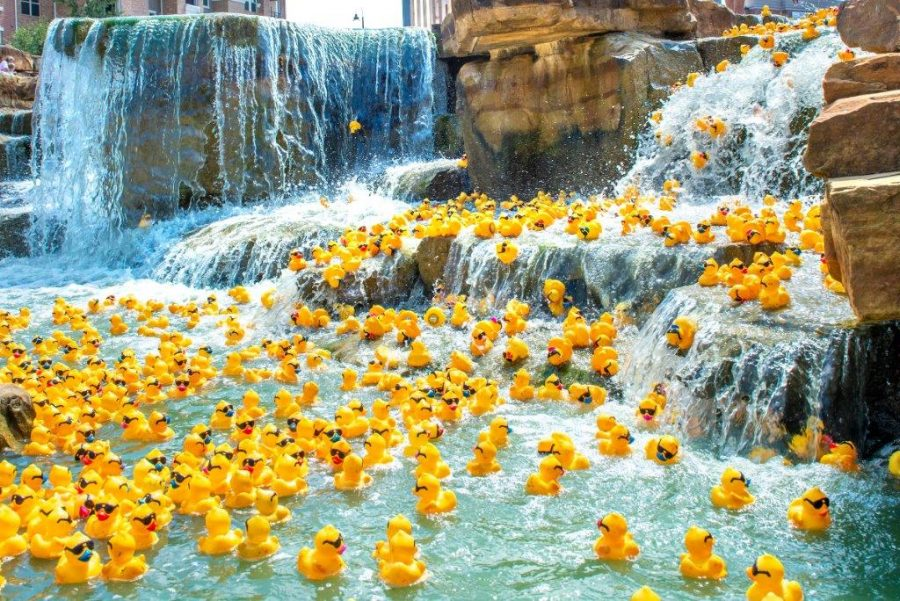
\includegraphics[width=0.75\textwidth]{/Users/ruipreis/Documents/Projects/obsitex/samples/images/ducks.png}
\caption{Example of a duck city}
\end{figure}


A random reference \citep{weiFinetunedLanguageModels2022}.

\chapter{Literature Review}\label{sec:Literature_Review}

Although there is no direct research on duck-sized horses, literature on miniature animals in urban settings provides a foundation for analysis. Studies on therapy animals, micro-livestock, and unconventional pets help frame the discussion. Additionally, urban ecology research highlights the potential environmental implications of introducing new species, even those that are artificially scaled down.



\begin{table}[H]
\centering
\caption{Comparison of Various Duck Species, Their Habitats, Lifespans, and Unique Features.}
\begin{tabular}{lrrr}
\toprule
Duck Species & Habitat & Average Lifespan & Notable Feature \\
\midrule
Mallard & Lakes, Ponds, Rivers & 5-10 years & Iridescent green head (males) \\
Wood Duck & Forested Wetlands & 3-4 years & Perches in trees, colorful plumage \\
Mandarin Duck & East Asian Lakes & 6-7 years & Striking multicolored feathers \\
Muscovy Duck & Swamps, Farms & 8-12 years & Red facial caruncles \\
Eider Duck & Coastal Waters & 15-20 years & Soft down feathers used in insulation \\
Pekin Duck & Domestic/Farms & 5-9 years & Popular breed for duck farming \\
Harlequin Duck & Rocky Coastal Streams & 10-12 years & Distinctive black and white markings \\
\bottomrule
\end{tabular}
\end{table}


\chapter{Methodology}\label{sec:Methodology}

A mixed-methods approach is employed to assess the theoretical integration of duck-sized horses in urban settings. This includes:



\begin{itemize}
	\item \textbf{Surveys}: Conducted among urban dwellers to gauge perceptions of miniature horses in public spaces.
	\item \textbf{Economic Simulations}: Modeled scenarios where duck-sized horses serve as transportation aids, novelty attractions, or companion animals.
	\item \textbf{Comparative Analysis}: Examining historical cases of animal integration in cities, such as working horses in early industrial societies and modern urban beekeeping initiatives.
\end{itemize}


\part{Findings and Implications}\label{sec:Findings_and_Implications}

\chapter{Findings and Discussion}\label{sec:Findings_and_Discussion}

\section{Economic Viability}\label{sec:Economic_Viability}

Duck-sized horses could have multiple economic applications, such as serving as novelty pets, therapy animals, or even eco-friendly alternatives to scooters in pedestrian zones. However, concerns arise regarding their care, maintenance costs, and the regulatory framework needed to manage them in high-density areas.

\section{Social and Cultural Implications}\label{sec:Social_and_Cultural_Implications}

Public opinion appears divided on the integration of duck-sized horses into urban environments. While some respondents express enthusiasm for their potential as stress-relief animals, others raise concerns about their impact on sanitation, noise levels, and the risk of displacement of existing urban species.

\section{Urban Planning and Infrastructure Challenges}\label{sec:Urban_Planning_and_Infrastructure_Challenges}

Adapting urban spaces to accommodate duck-sized horses would require modifications to sidewalks, public transport systems, and waste management practices. Issues such as designated grazing areas and water access points also emerge as critical considerations.

\chapter{Conclusion}\label{sec:Conclusion}

While the concept of duck-sized horses in urban environments is largely hypothetical, its exploration reveals deeper insights into how cities accommodate non-human life. If such creatures were ever introduced, their economic, social, and infrastructural implications would need to be carefully managed to ensure harmonious integration. Future research may explore the feasibility of genetic engineering to create scalable urban livestock tailored to specific needs.


\bibliography{main}                         


\printindex

\pagestyle{empty}
\cleartoevenpage
\null
\thispagestyle{empty}
\pagecolor{PANTONECoolGray7C}
\afterpage{\nopagecolor}
\newpage

\begin{backcover}
\thispagestyle{empty}{~\vfill
\noindent
% Place here information about funding, FCT project, etc. in which the work is framed. Leave empty otherwise.
\vfill ~}
\end{backcover}



\end{document}
